\documentclass[CJK]{beamer}
\usepackage{cleveref}

\usepackage{CJKutf8}
\usepackage{beamerthemesplit}
\usetheme{Malmoe}
\useoutertheme[footline=authortitle]{miniframes}
\usepackage{amsmath}
\usepackage{amssymb}
\usepackage{graphicx}
\usepackage{eufrak}
\usepackage{color}
\usepackage{slashed}
\usepackage{simplewick}
\usepackage{tikz}
\usepackage{tcolorbox}
\graphicspath{{../figures/}}
%%figures
\def\lfig#1#2{\includegraphics[width=#1 in]{#2}}
\def\addfig#1#2{\begin{center}\includegraphics[width=#1 in]{#2}\end{center}}
\def\wulian{\includegraphics[width=0.18in]{emoji_wulian.jpg}}
\def\bigwulian{\includegraphics[width=0.35in]{emoji_wulian.jpg}}
\def\bye{\includegraphics[width=0.18in]{emoji_bye.jpg}}
\def\bigbye{\includegraphics[width=0.35in]{emoji_bye.jpg}}
\def\huaixiao{\includegraphics[width=0.18in]{emoji_huaixiao.jpg}}
\def\bighuaixiao{\includegraphics[width=0.35in]{emoji_huaixiao.jpg}}
\def\jianxiao{\includegraphics[width=0.18in]{emoji_jianxiao.jpg}}
\def\bigjianxiao{\includegraphics[width=0.35in]{emoji_jianxiao.jpg}}
%% colors
\def\blacktext#1{{\color{black}#1}}
\def\bluetext#1{{\color{blue}#1}}
\def\redtext#1{{\color{red}#1}}
\def\darkbluetext#1{{\color[rgb]{0,0.2,0.6}#1}}
\def\skybluetext#1{{\color[rgb]{0.2,0.7,1.}#1}}
\def\cyantext#1{{\color[rgb]{0.,0.5,0.5}#1}}
\def\greentext#1{{\color[rgb]{0,0.7,0.1}#1}}
\def\darkgray{\color[rgb]{0.2,0.2,0.2}}
\def\lightgray{\color[rgb]{0.6,0.6,0.6}}
\def\gray{\color[rgb]{0.4,0.4,0.4}}
\def\blue{\color{blue}}
\def\red{\color{red}}
\def\green{\color{green}}
\def\darkgreen{\color[rgb]{0,0.4,0.1}}
\def\darkblue{\color[rgb]{0,0.2,0.6}}
\def\skyblue{\color[rgb]{0.2,0.7,1.}}
%%control
\def\be{\begin{equation}}
\def\ee{\nonumber\end{equation}}
\def\bea{\begin{eqnarray}}
\def\eea{\nonumber\end{eqnarray}}
\def\bch{\begin{CJK}{UTF8}{gbsn}}
\def\ech{\end{CJK}}
\def\bitem{\begin{itemize}}
\def\eitem{\end{itemize}}
\def\bcenter{\begin{center}}
\def\ecenter{\end{center}}
\def\bex{\begin{minipage}{0.2\textwidth}\includegraphics[width=0.6in]{jugelizi.png}\end{minipage}\begin{minipage}{0.76\textwidth}}
\def\eex{\end{minipage}}
\def\chtitle#1{\frametitle{\bch#1\ech}}
\def\bmat#1{\left(\begin{array}{#1}}
\def\emat{\end{array}\right)}
\def\bcase#1{\left\{\begin{array}{#1}}
\def\ecase{\end{array}\right.}
\def\bmini#1{\begin{minipage}{#1\textwidth}}
\def\emini{\end{minipage}}
\def\tbox#1{\begin{tcolorbox}#1\end{tcolorbox}}
\def\pfrac#1#2#3{\left(\frac{\partial #1}{\partial #2}\right)_{#3}}
%%symbols
\def\bropt{\,(\ \ \ )}
\def\sone{$\star$}
\def\stwo{$\star\star$}
\def\sthree{$\star\star\star$}
\def\sfour{$\star\star\star\star$}
\def\sfive{$\star\star\star\star\star$}
\def\rint{{\int_\leftrightarrow}}
\def\roint{{\oint_\leftrightarrow}}
\def\stdHf{{\textit{\r H}_f}}
\def\deltaH{{\Delta \textit{\r H}}}
\def\ii{{\dot{\imath}}}
\def\skipline{{\vskip0.1in}}
\def\skiplines{{\vskip0.2in}}
\def\lagr{{\mathcal{L}}}
\def\hamil{{\mathcal{H}}}
\def\vecv{{\mathbf{v}}}
\def\vecx{{\mathbf{x}}}
\def\vecy{{\mathbf{y}}}
\def\veck{{\mathbf{k}}}
\def\vecp{{\mathbf{p}}}
\def\vecn{{\mathbf{n}}}
\def\vecA{{\mathbf{A}}}
\def\vecP{{\mathbf{P}}}
\def\vecsigma{{\mathbf{\sigma}}}
\def\hatJn{{\hat{J_\vecn}}}
\def\hatJx{{\hat{J_x}}}
\def\hatJy{{\hat{J_y}}}
\def\hatJz{{\hat{J_z}}}
\def\hatj#1{\hat{J_{#1}}}
\def\hatphi{{\hat{\phi}}}
\def\hatq{{\hat{q}}}
\def\hatpi{{\hat{\pi}}}
\def\vel{\upsilon}
\def\Dint{{\mathcal{D}}}
\def\adag{{\hat{a}^\dagger}}
\def\bdag{{\hat{b}^\dagger}}
\def\cdag{{\hat{c}^\dagger}}
\def\ddag{{\hat{d}^\dagger}}
\def\hata{{\hat{a}}}
\def\hatb{{\hat{b}}}
\def\hatc{{\hat{c}}}
\def\hatd{{\hat{d}}}
\def\hatN{{\hat{N}}}
\def\hatH{{\hat{H}}}
\def\hatp{{\hat{p}}}
\def\Fup{{F^{\mu\nu}}}
\def\Fdown{{F_{\mu\nu}}}
\def\newl{\nonumber \\}
\def\vece{\mathrm{e}}
\def\calM{{\mathcal{M}}}
\def\calT{{\mathcal{T}}}
\def\calR{{\mathcal{R}}}
\def\barpsi{\bar{\psi}}
\def\baru{\bar{u}}
\def\barv{\bar{\upsilon}}
\def\qeq{\stackrel{?}{=}}
\def\torder#1{\mathcal{T}\left(#1\right)}
\def\rorder#1{\mathcal{R}\left(#1\right)}
\def\contr#1#2{\contraction{}{#1}{}{#2}#1#2}
\def\trof#1{\mathrm{Tr}\left(#1\right)}
\def\trace{\mathrm{Tr}}
\def\comm#1{\ \ \ \left(\mathrm{used}\ #1\right)}
\def\tcomm#1{\ \ \ (\text{#1})}
\def\slp{\slashed{p}}
\def\slk{\slashed{k}}
\def\calp{{\mathfrak{p}}}
\def\veccalp{\mathbf{\mathfrak{p}}}
\def\Tthree{T_{\tiny \textcircled{3}}}
\def\pthree{p_{\tiny \textcircled{3}}}
\def\dbar{{\,\mathchar'26\mkern-12mu d}}
\def\erf{\mathrm{erf}}
\def\const{\mathrm{constant}}
\def\pheat{\pfrac p{\ln T}V}
\def\vheat{\pfrac V{\ln T}p}
%%units
\def\fdeg{{^\circ \mathrm{F}}}
\def\cdeg{^\circ \mathrm{C}}
\def\atm{\,\mathrm{atm}}
\def\angstrom{\,\text{\AA}}
\def\SIL{\,\mathrm{L}}
\def\SIkm{\,\mathrm{km}}
\def\SIyr{\,\mathrm{yr}}
\def\SIGyr{\,\mathrm{Gyr}}
\def\SIV{\,\mathrm{V}}
\def\SImV{\,\mathrm{mV}}
\def\SIeV{\,\mathrm{eV}}
\def\SIkeV{\,\mathrm{keV}}
\def\SIMeV{\,\mathrm{MeV}}
\def\SIGeV{\,\mathrm{GeV}}
\def\SIcal{\,\mathrm{cal}}
\def\SIkcal{\,\mathrm{kcal}}
\def\SImol{\,\mathrm{mol}}
\def\SIN{\,\mathrm{N}}
\def\SIHz{\,\mathrm{Hz}}
\def\SIm{\,\mathrm{m}}
\def\SIcm{\,\mathrm{cm}}
\def\SIfm{\,\mathrm{fm}}
\def\SImm{\,\mathrm{mm}}
\def\SInm{\,\mathrm{nm}}
\def\SImum{\,\mathrm{\mu m}}
\def\SIJ{\,\mathrm{J}}
\def\SIW{\,\mathrm{W}}
\def\SIkJ{\,\mathrm{kJ}}
\def\SIs{\,\mathrm{s}}
\def\SIkg{\,\mathrm{kg}}
\def\SIg{\,\mathrm{g}}
\def\SIK{\,\mathrm{K}}
\def\SImmHg{\,\mathrm{mmHg}}
\def\SIPa{\,\mathrm{Pa}}


\newcommand{\field}{\mathscr{F}}

\newcommand{\reals}{\mathbb{R}}
\newcommand{\complexs}{\mathbb{C}}
\newcommand{\ints}{\mathbb{Z}}
%\newcommand{\dim}{\mathrm{dim\ }}
\newcommand{\diag}{\mathrm{diag \ }}
\newcommand{\up}{\uparrow}
\newcommand{\down}{\downarrow}
\newcommand{\su}{\mathfrak{su}}
\newcommand{\so}{\mathfrak{so}}
\newcommand{\tr}{\mathrm{tr\ }}
\newcommand{\card}{\mathrm{card \ }}
\newcommand{\unit}[1]{\mathrm{\ #1}}
\def\secpage#1#2{\begin{frame}\bch\bcenter{\bf \Huge #1} \skipline \tbox{#2}\ecenter\ech\end{frame}}
\newtheorem{thm}{定理}[section]
\newtheorem{axm}{公理}[section]
\newtheorem{dfn}{定义}[section]

\crefname{figure}{图}{图}

%\cpic{<尺寸>}{<文件名>}}用于生成居中的图片。
\newcommand{\cpic}[2]{
\begin{center}
\includegraphics[scale=#1]{#2}
\end{center}
}

%\cpicn{<尺寸>}{<文件名>}{<注释>}用于生成居中且带有注释的图片,其label为图片名。
\newcommand{\cpicn}[3]
{
\begin{figure}[h!]
\cpic{#1}{#2}
\caption{#3\label{#2}}
\end{figure}
}

\title{Applications of Quantum Mechanics\\ Chapter 2-Band Structure}
  \author{}
  \date{}


\begin{document}

\begin{frame}
\frametitle{\bch 欢迎您,走进 \ech}
\bch
凝聚态物理学的殿堂
\cpic{0.55}{whopper}
\ech
\end{frame}


\begin{frame}
 
\begin{center}
\begin{Large}
\bch
{\bf Applications of Quantum Mechanics}

{\vskip 0.3in}

Chapter 2-Band Structure

\ech
\end{Large}
\end{center}

\vskip 0.2in
\begin{center}
Han Gao
\vskip 0.1in
gaoh26@mail2.sysu.edu.cn
\vskip 0.2in
Zonglin Mo
\vskip 0.1in
mozlin@mail2.sysu.edu.cn
\vskip 0.2in

\end{center}


\end{frame}

\section{Condensed Matter}
\begin{frame}
\frametitle{\bch 凝聚态物理学的研究对象 \ech}
\bch
以下是一位著名凝聚态物理学专家近年发表的一些文章标题:
\emph{
\begin{itemize}
\item Field-Free Deterministic Magnetization Switching with Ultralow Current Density in Epitaxial ${\rm Au/Fe_4N}$ Bilayer Films
\item Performance of Inverted Quantum Dot Light-Emitting Diodes Enhanced by Using Phosphorescent Molecules as Exciton Harvesters
\item Influence of electron transport layer thickness on optical properties of organic light emitting diodes
\item High efficiency electrophosphorescent organic light-emitting diodes with double light-emitting layers
\end{itemize}
}
阅读上面的标题,你认为凝聚态物理学的研究对象和方法是什么?
\ech
\end{frame}



\begin{frame}
\frametitle{\bch 凝聚态物理学 \ech}
\bch
凝聚态物理学主要研究固体材料的导电、导热、光学性质。
\par
凝聚态物理学的研究方法和大多数物理分支一样,也是理论和\begin{LARGE} {\bf 实验 } \end{LARGE}。
\begin{figure}[h!]
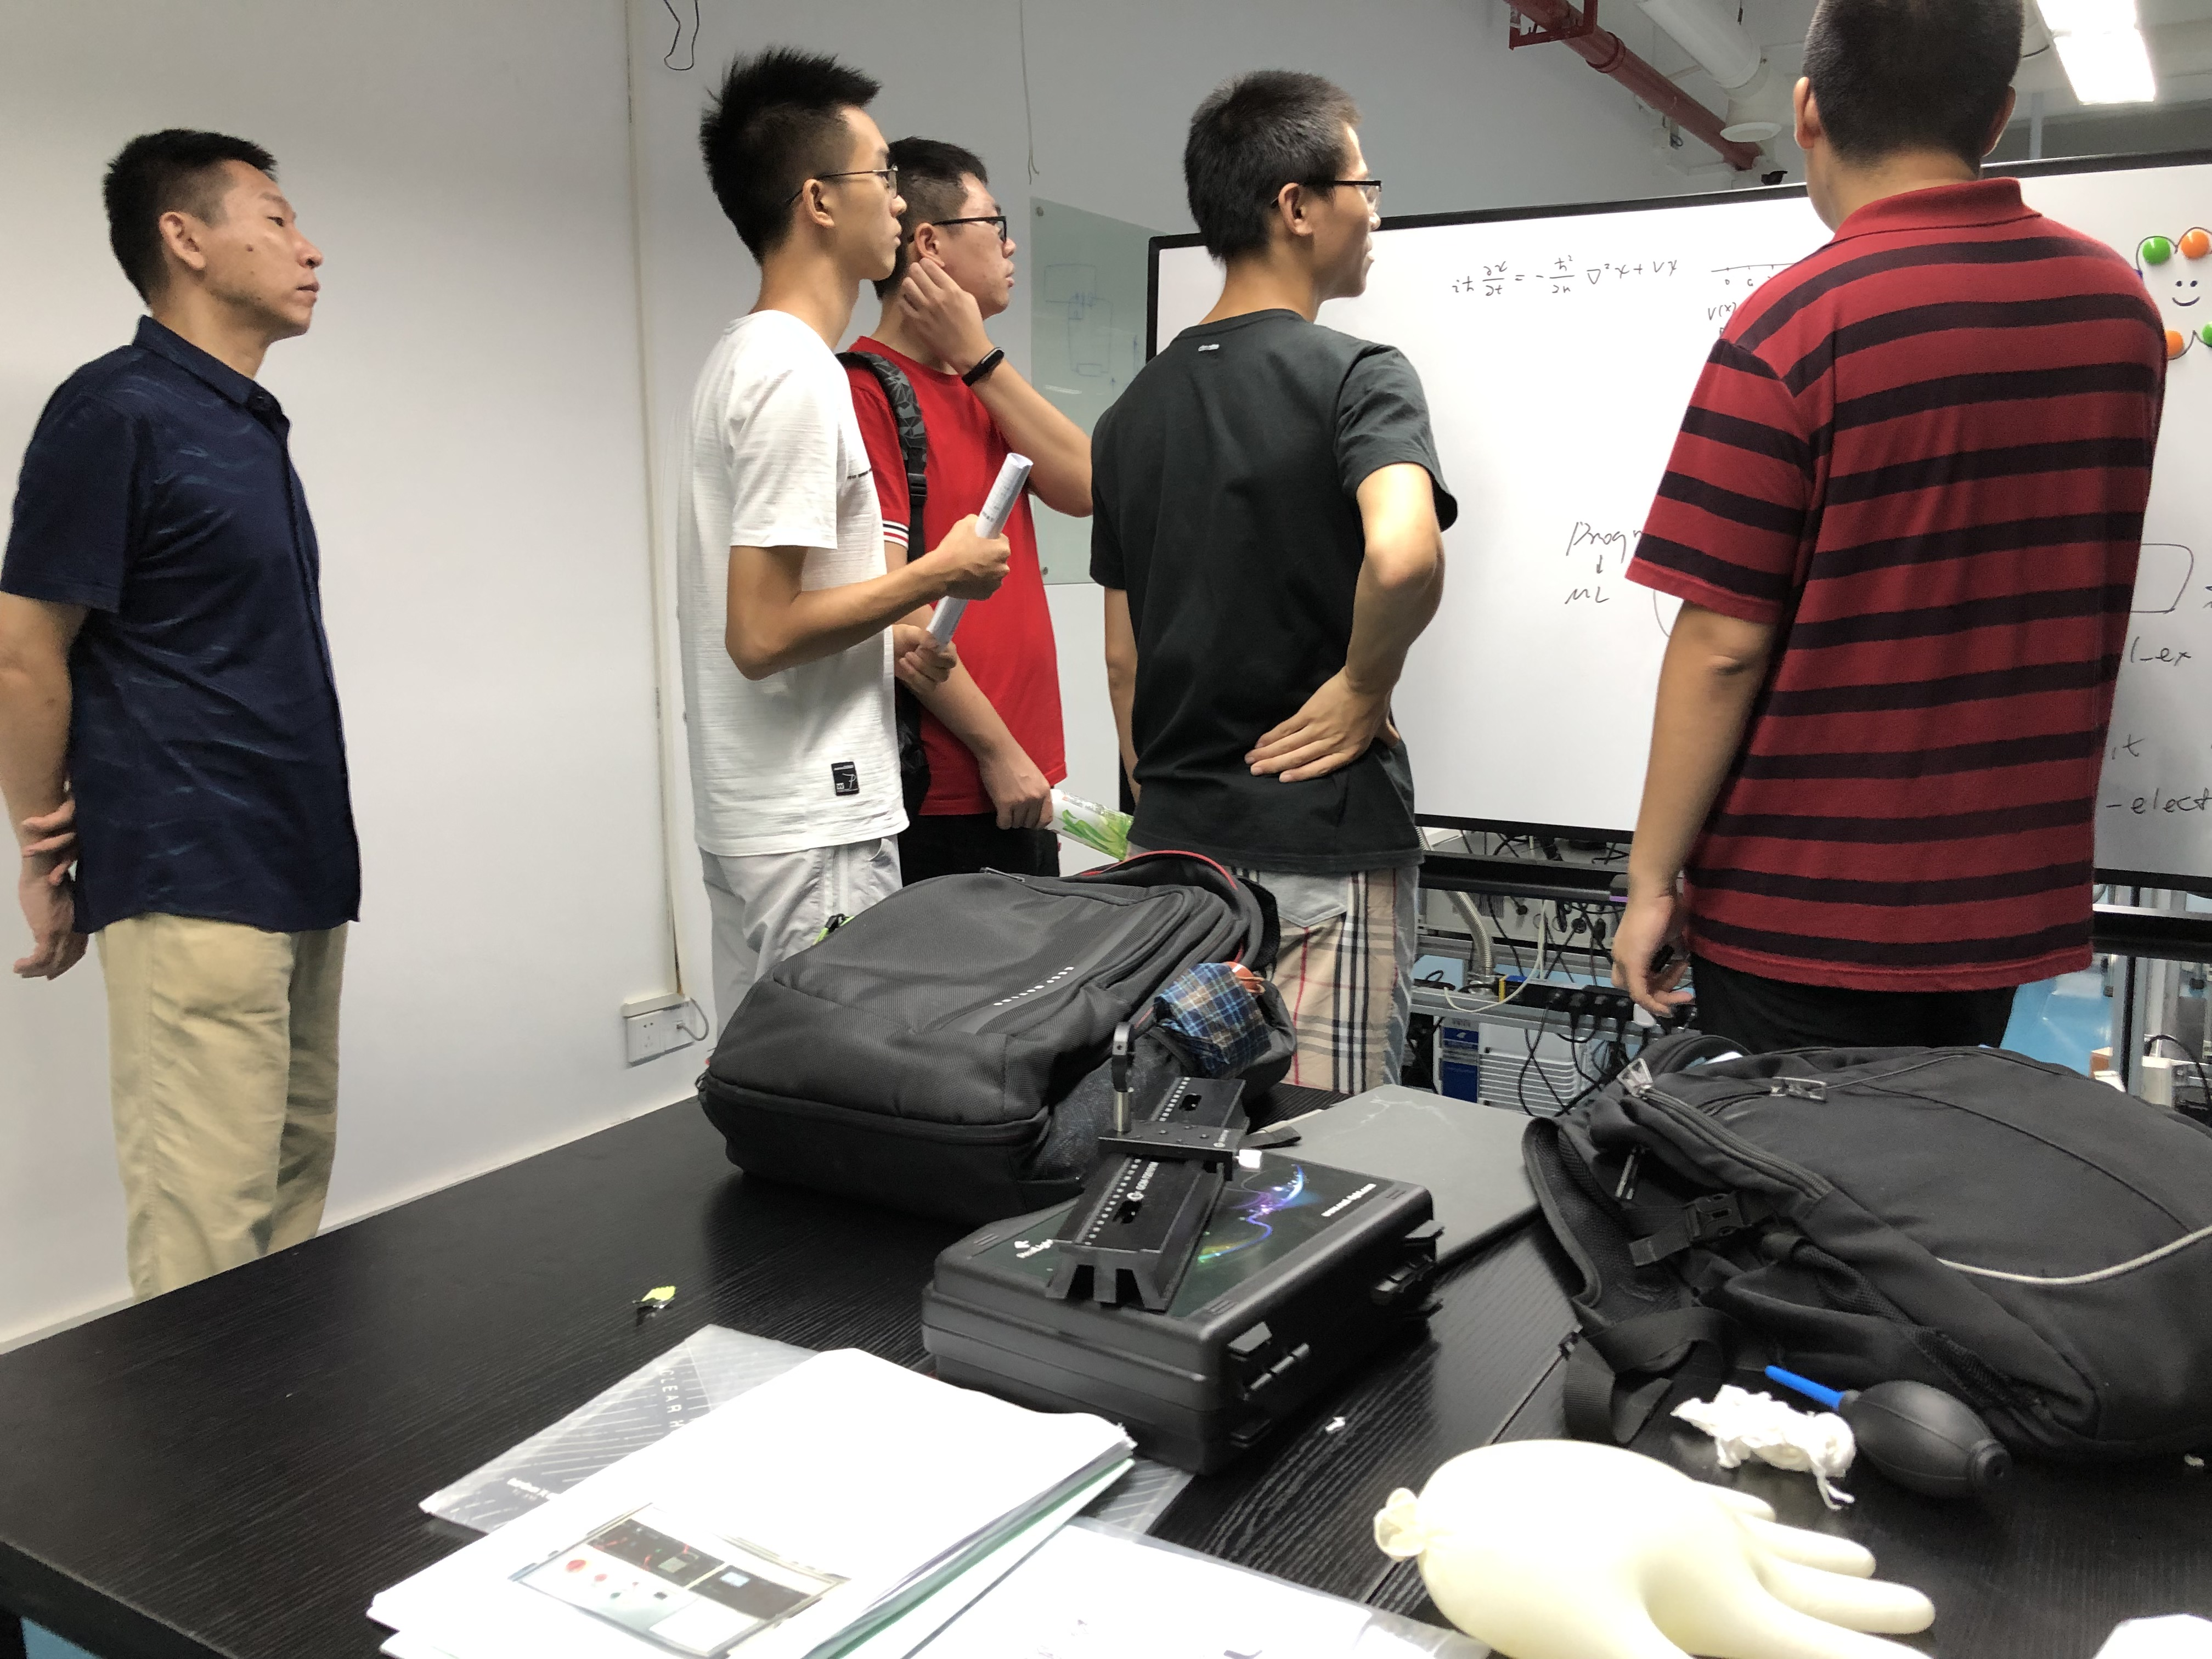
\includegraphics[scale=0.028]{theory}
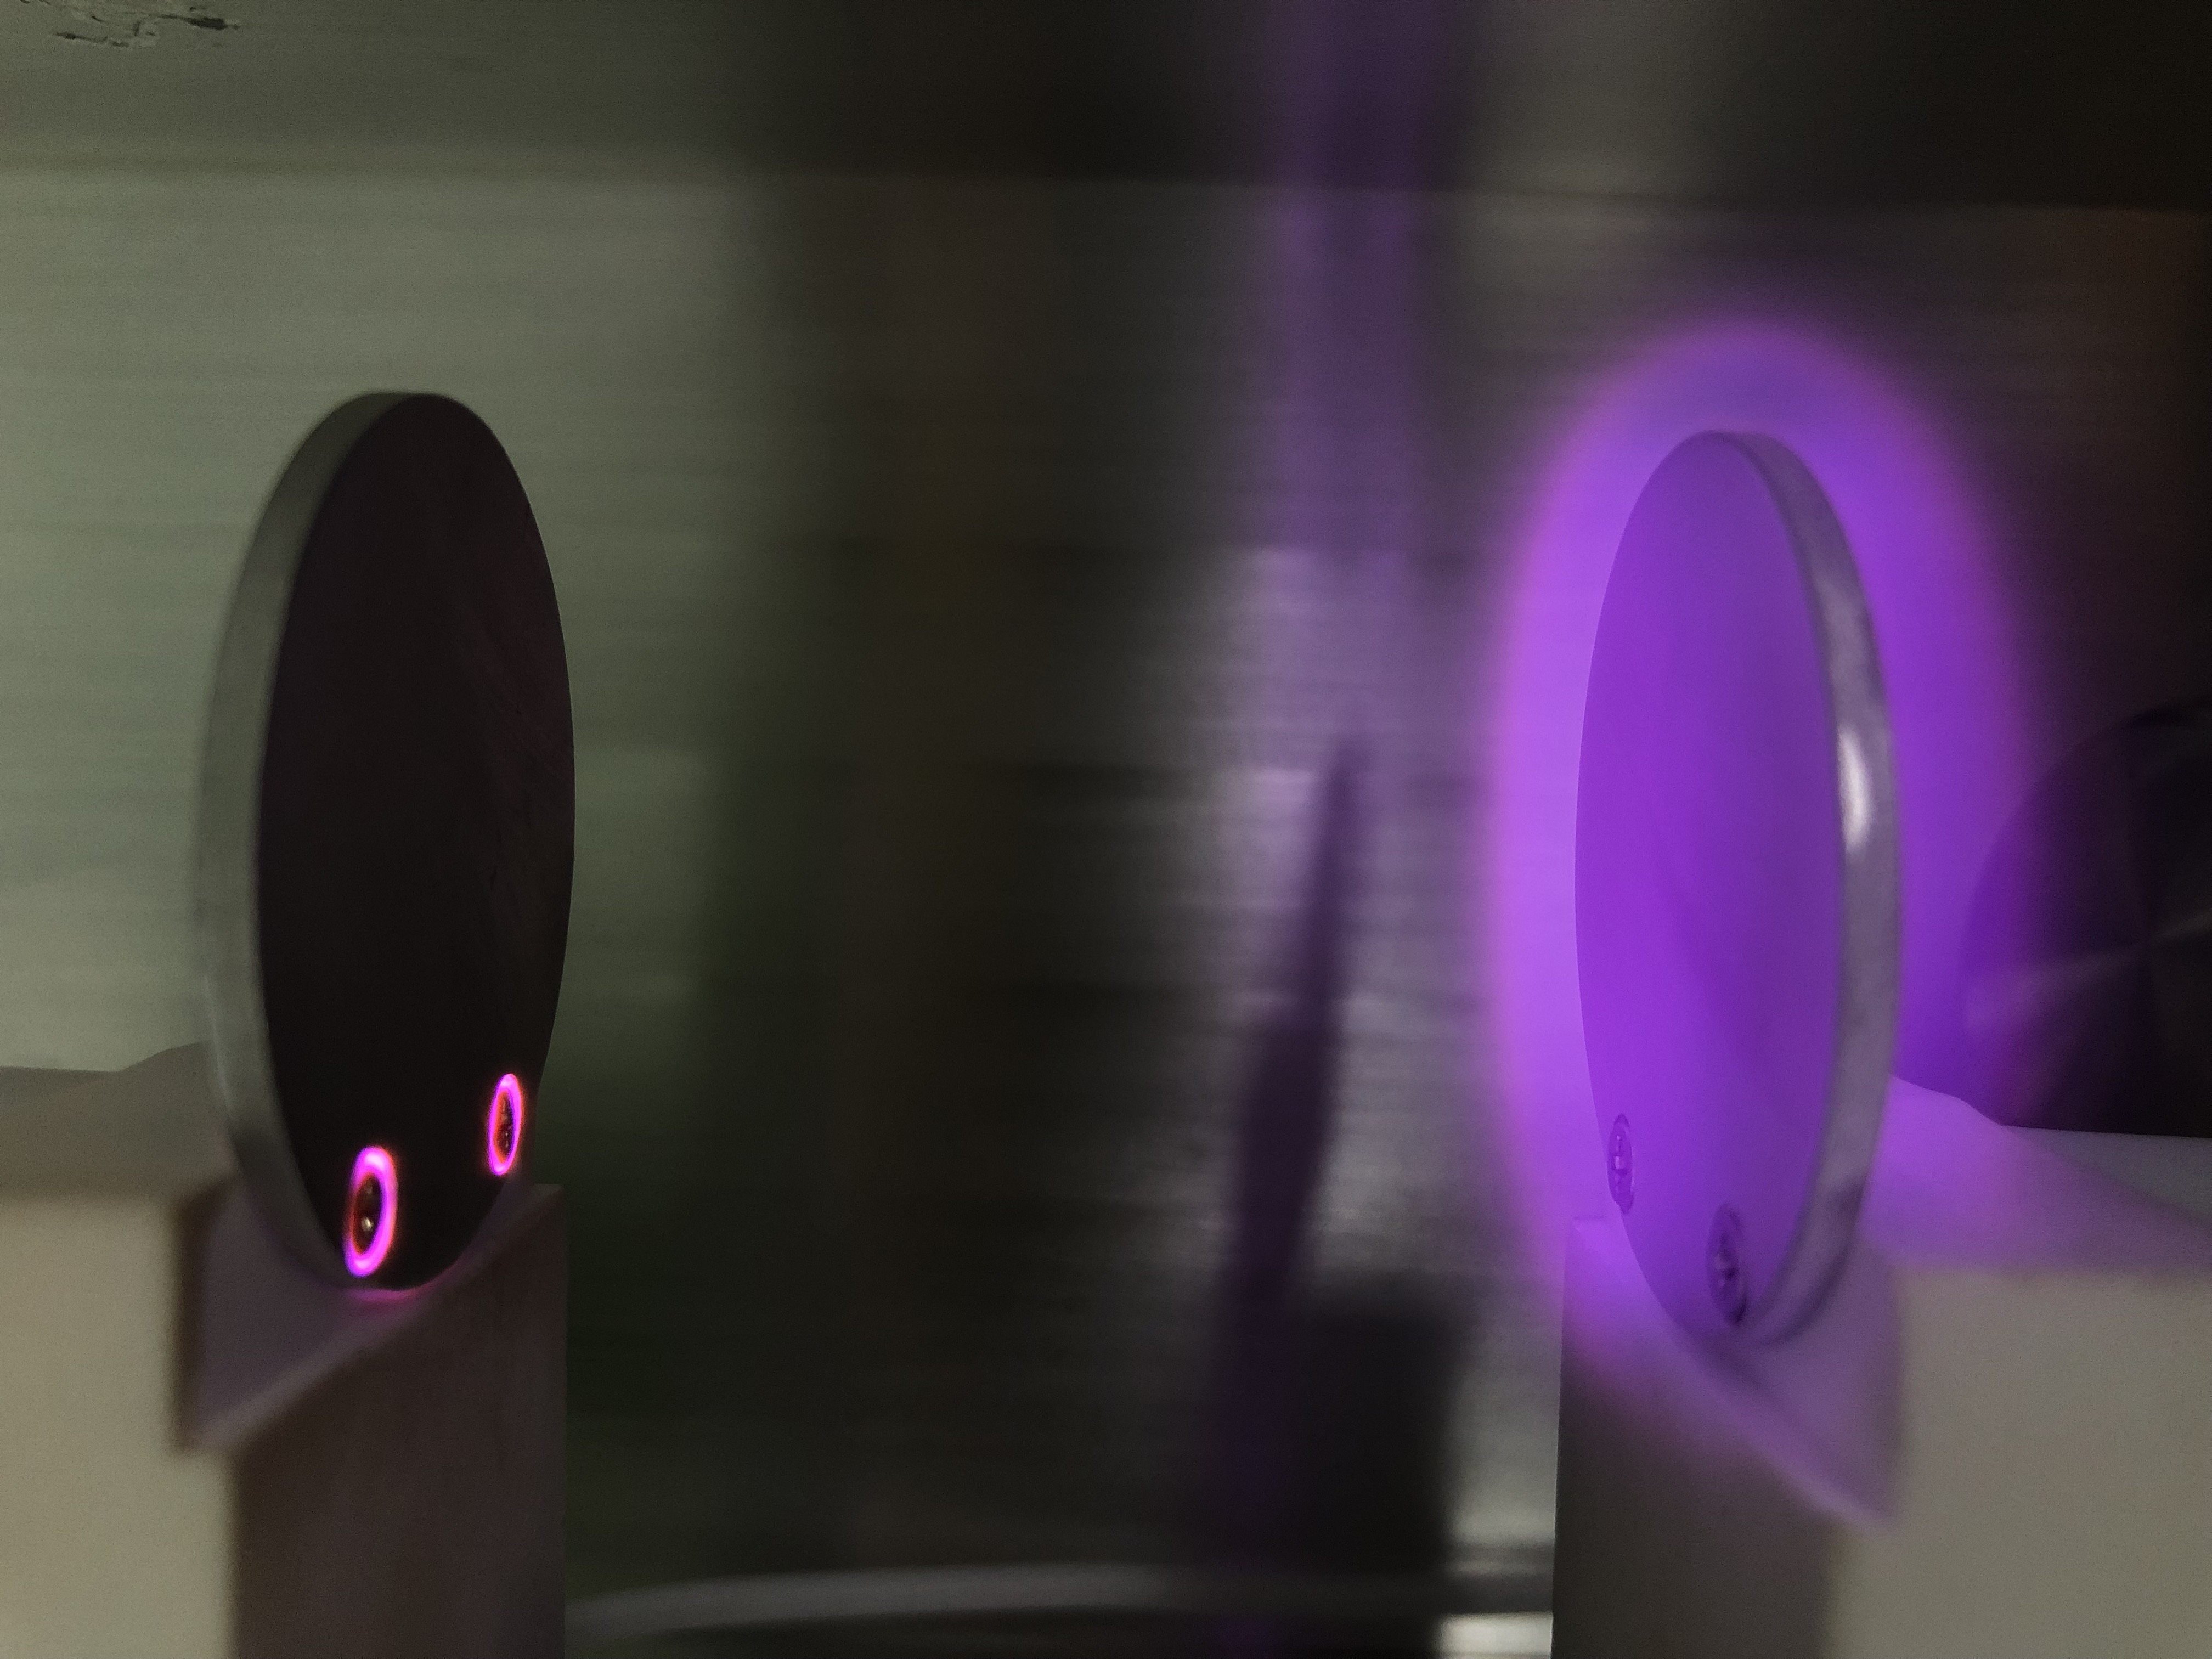
\includegraphics[scale=0.028]{expe}
\caption{凝聚态物理理论探究(左)和实验(右)}
\end{figure}
\ech
\end{frame}

\begin{frame}
\frametitle{\bch 无处不在的凝聚态 \ech}
\bch
\cpic{0.035}{nanchang}
绚丽多彩的{\bf 南昌}之星摩天轮(上左)的霓虹灯,凝聚态物理学研究物质的光学性质。
\ech
\end{frame}

\begin{frame}
\frametitle{\bch 无处不在的凝聚态 \ech}
\bch
\cpic{0.05}{chengdu}
{\bf 成都}双流机场机坪上的A350客机,飞机的研发制造需要寻找轻盈耐腐蚀的材料,凝聚态物理学研究材料的表面性质。
\ech
\end{frame}

\begin{frame}
\frametitle{\bch 无处不在的凝聚态 \ech}
\bch
\cpic{0.05}{shanghai}
从{\bf 上海}外滩看陆家嘴的灯光,凝聚态物理学研究材料的光学和电学性质,从而使得灯火更加灿烂。
\ech
\end{frame}


\begin{frame}
\frametitle{\bch 格点 Lattice \ech}
\bch
由于固体的微观周期性,原子生活在格点上,而电子在以格点划分的区域间运动。\par
场论中也常常用到Lattice化的方法,进行公式推导和第一性原理计算。场论和凝聚态的研究手段常有互相借鉴。
\ech
\end{frame}

\begin{frame}
\frametitle{\bch 周期性边界条件 \ech}
\bch
\begin{itemize}
\item 实际的固体很大,使得边界对固体性质的影响很小。为了削弱边界的影响以降低研究难度,我们常常假设边界性周期条件(PBC):
\item {\bf 设$N$为某个方向上的格点总数,要求标号$n$和$n+N$描述同一个格点。}
\item 图像上看,我们把一个一维的原子链首尾相接弯成了一个原子环,从而消灭了边界。
\end{itemize}
\cpic{0.19}{pbc}
有时也直接假设晶格有无限个来消除边界。
\ech
\end{frame}

\begin{frame}
\frametitle{\bch 表面 \ech}
\bch
固体的边界称为表面。\par
一般涉及表面的研究相当困难,这一部分的研究称为{\bf 表面物理}。上海市复旦大学有著名的{\bf 应用表面物理国家重点实验室},前面提到的凝聚态物理学专家博士期间曾在这个实验室做了许多重要工作。
\begin{figure}[h!]
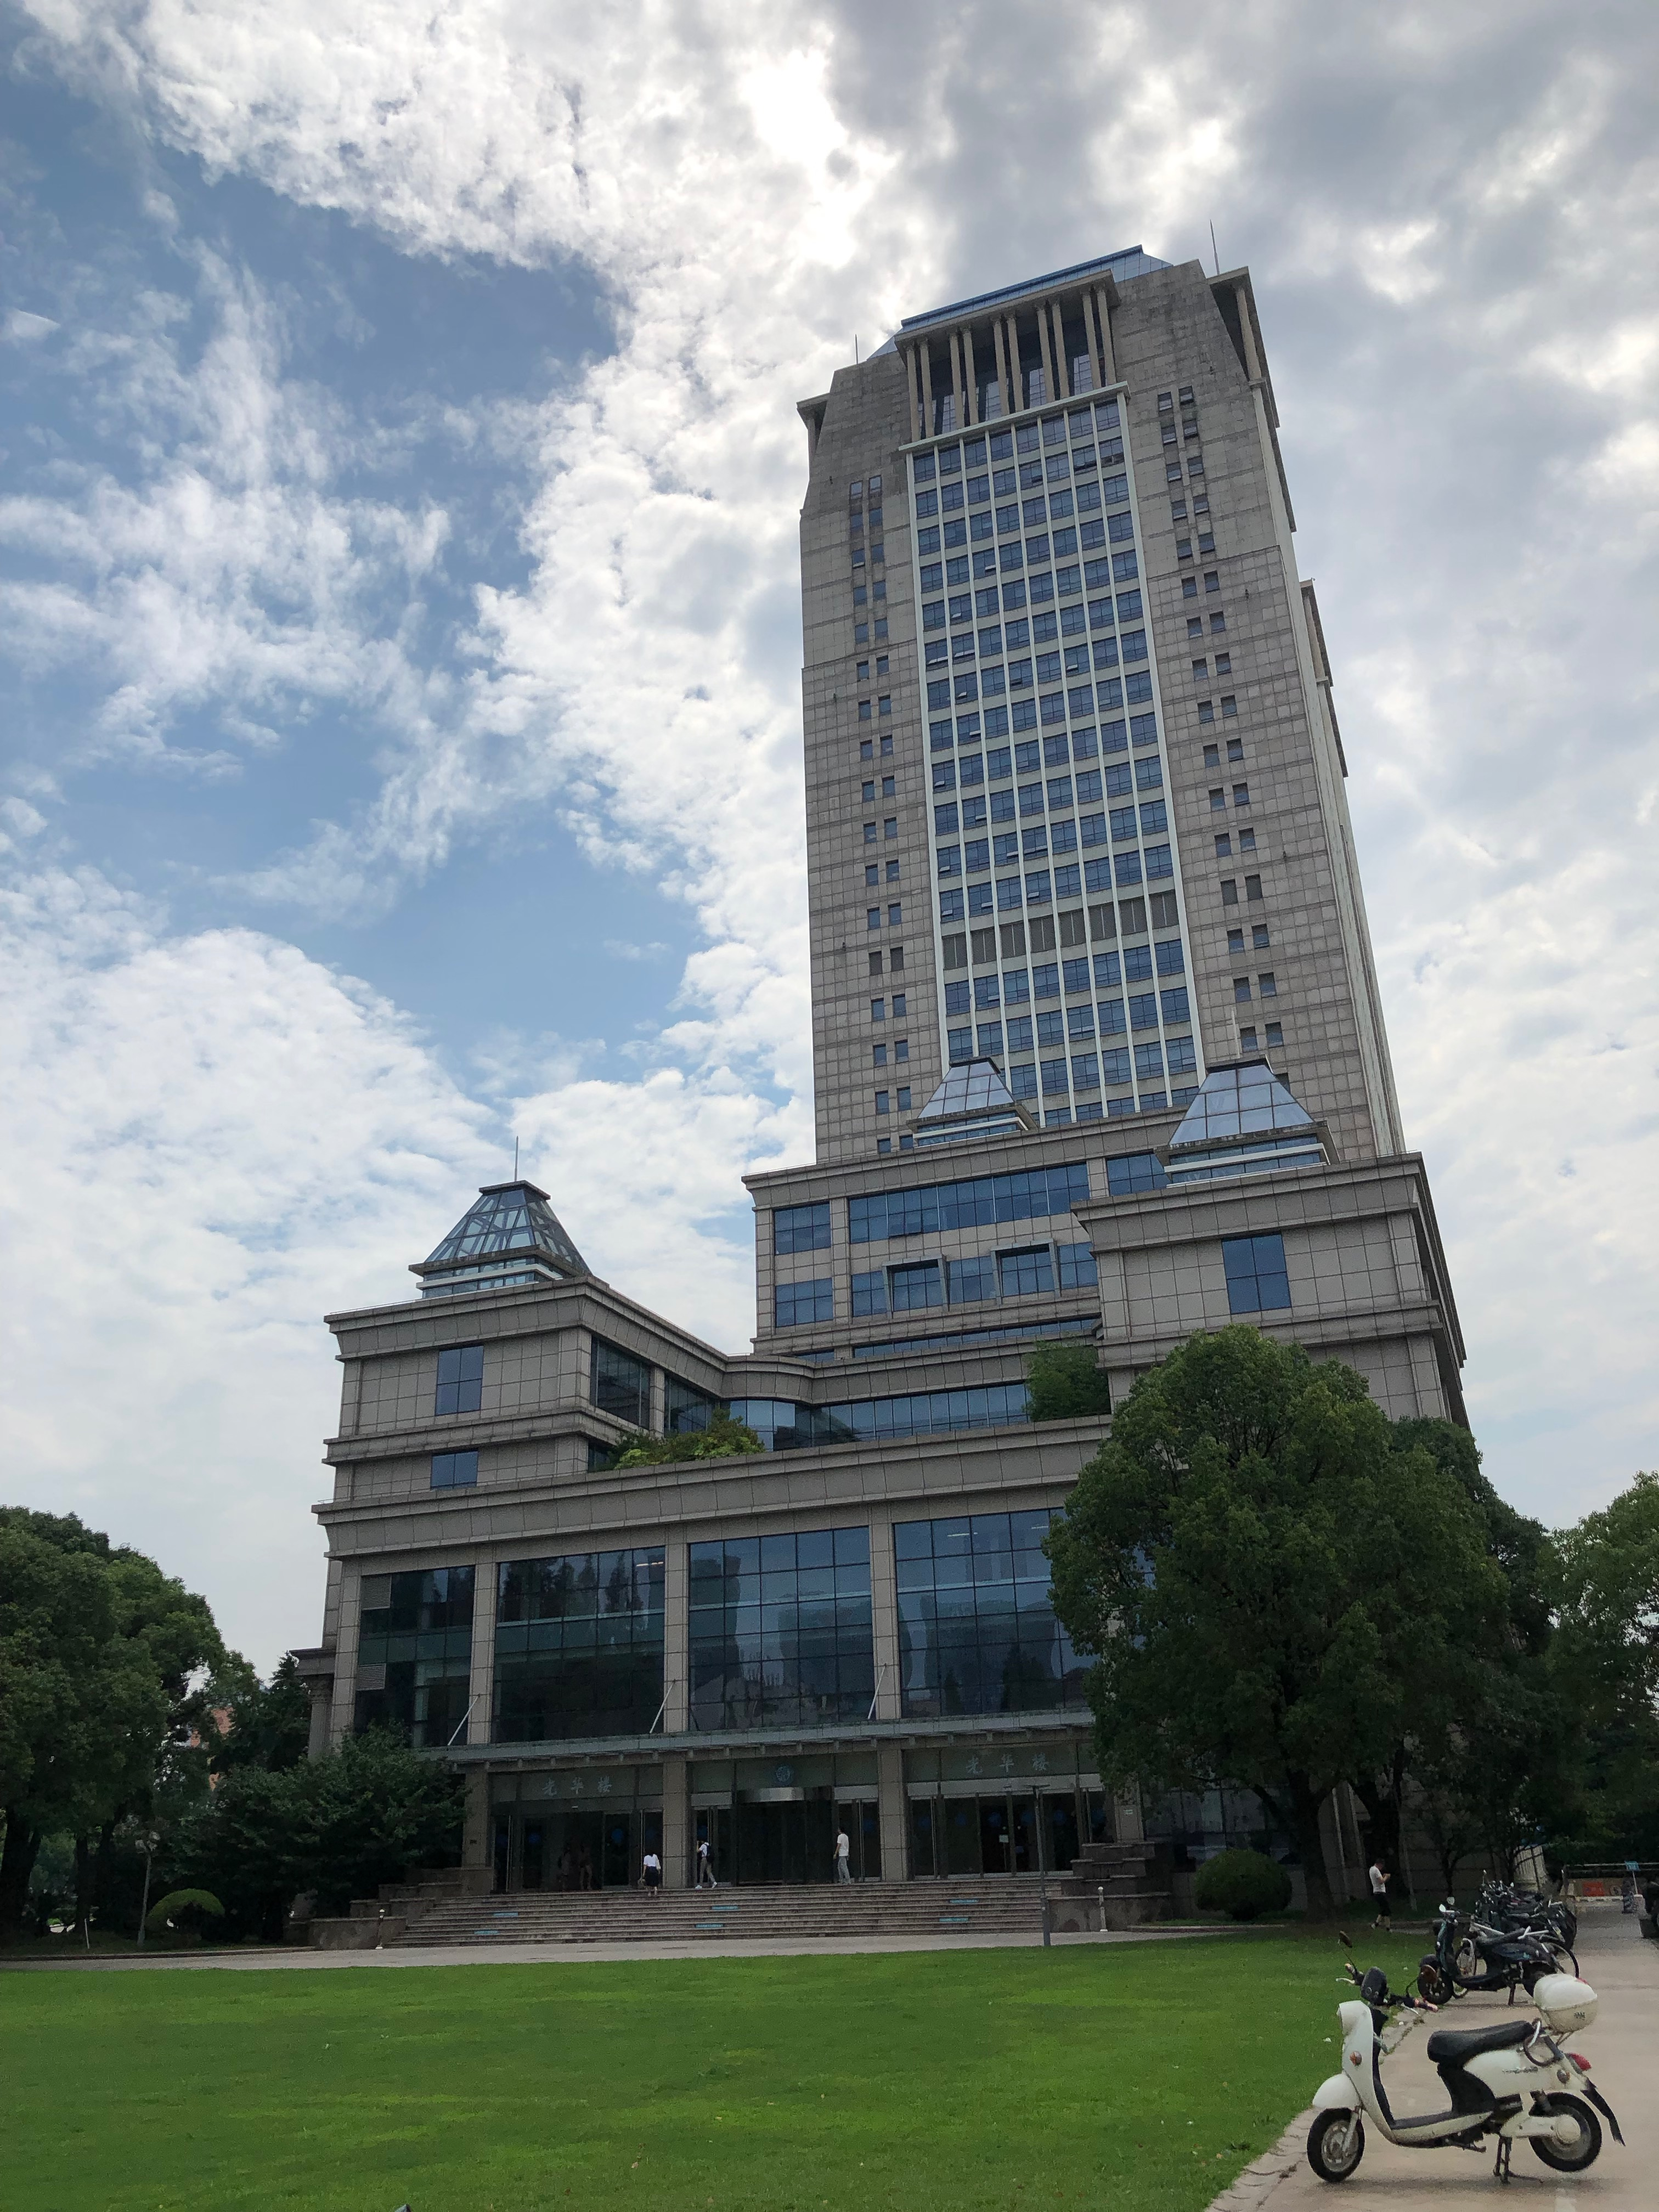
\includegraphics[scale=0.021]{fudan}
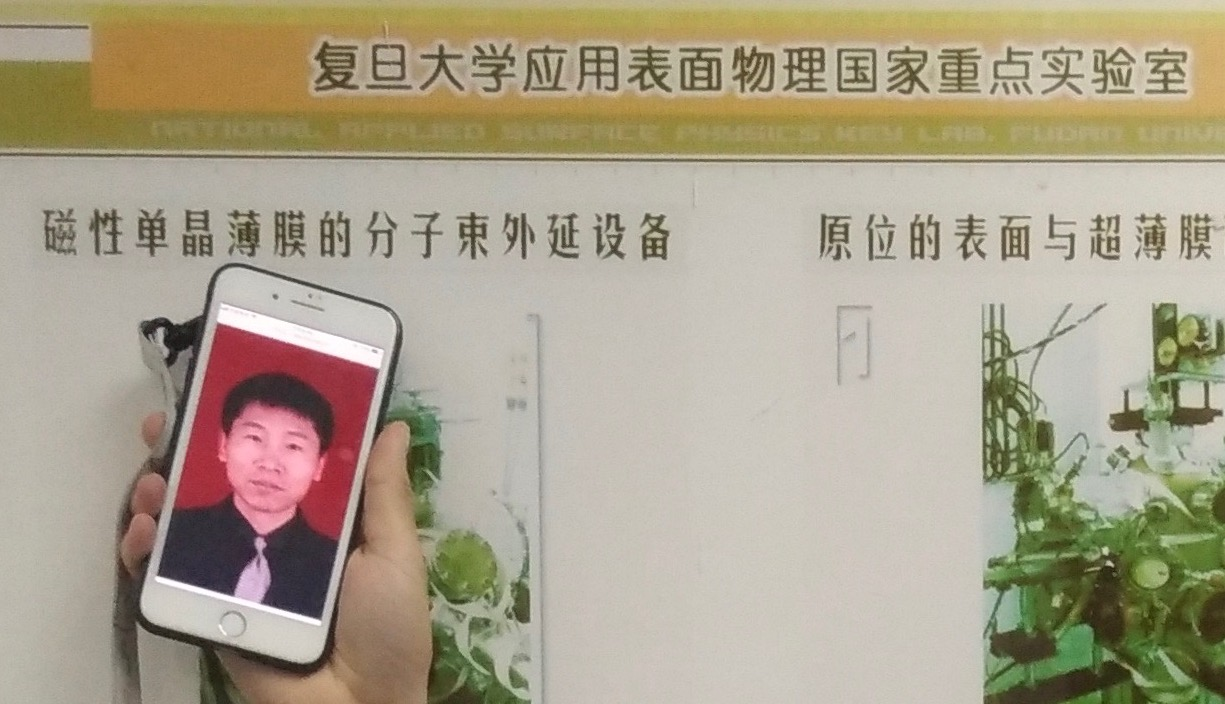
\includegraphics[scale=0.12]{surface}
\end{figure}
\ech
\end{frame}


\section{1D Models}

\secpage{一维固体模型}{离散平移对称性}

\begin{frame}
\frametitle{\bch 课堂互动:晶体 \ech}
\bch
你是选修三选手还是选修五选手?
\begin{figure}[h!]
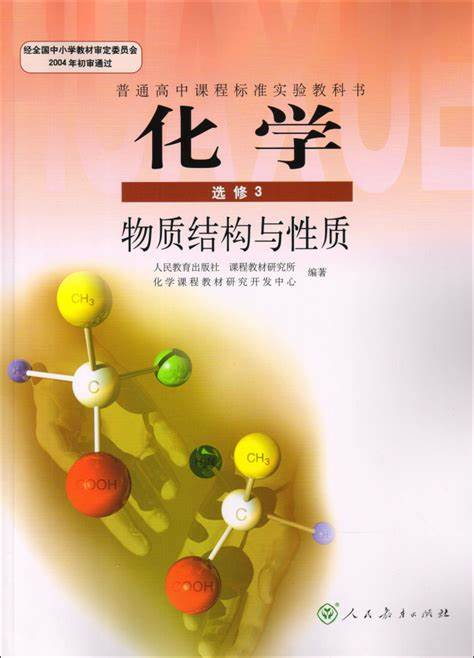
\includegraphics[scale=0.214]{chem3}
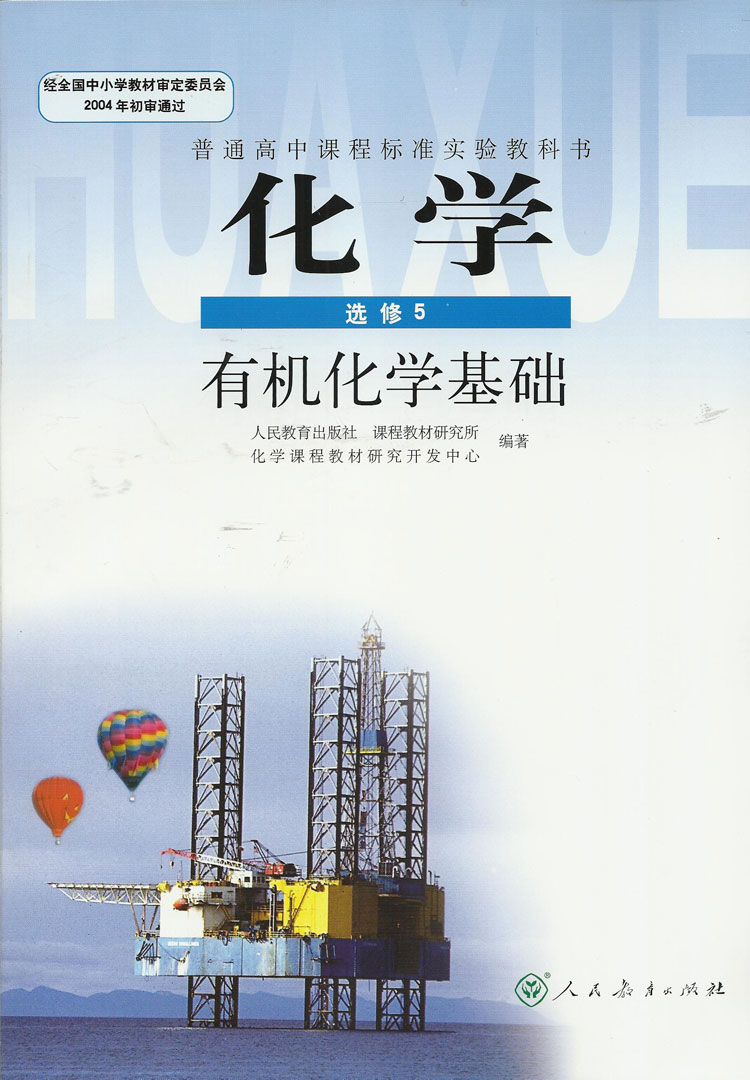
\includegraphics[scale=0.13]{chem5}
\end{figure}
\ech
\end{frame}

\begin{frame}
\frametitle{\bch 课堂互动:晶体 \ech}
\bch
请一位选修三选手为我们回顾一下离子晶体、原子晶体和金属晶体的基本图像。
\begin{figure}[h!]
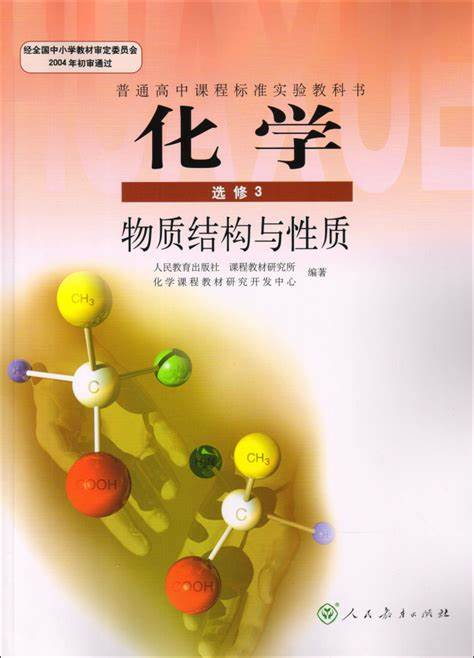
\includegraphics[scale=0.214]{chem3}

\end{figure}
\ech
\end{frame}

\begin{frame}
\frametitle{\bch 导电性 \ech}
\bch
向一个金属晶体入射电子,电子感受到的势场如何,电子将如何运动?
\ech
\end{frame}

\begin{frame}
\frametitle{\bch 一维束缚电子模型(TB模型) \ech}
\bch
假设电子被束缚在一维格点中,格点以$0,1,\cdots,n$标记,并有周期性边界条件。电子在第$n$格点的态记作$|n\rangle$。
\par
考虑哈密顿量
$$
H = -E_0 \sum_n |n \rangle \langle n | - t \sum_n \left( |n+1 \rangle \langle n | + |n\rangle \langle n+1 \rangle \right)
$$
第一项描述了电子在格点上的能量,第二项描述了电子在格点间可能的迁移。忽略了电子间的相互作用。
\ech
\end{frame}

\begin{frame}
\frametitle{\bch 本征方程 \ech}
\bch
一般电子的波函数按$|n\rangle$为基展开。
$$
| \psi \rangle = \psi_m |m \rangle
$$
哈密顿量对应的本征方程$H |\psi \rangle = E | \psi \rangle$。
\par
试证明,分量满足的薛定谔方程为
$$
-E_0 \psi_n - t (\psi_{n-1} + \psi_{n+1} ) = E\psi_n
$$
怎么求解这个方程呢?
\ech
\end{frame}


\begin{frame}
\frametitle{\bch 离散傅立叶变换 \ech}
\bch
上式难以求解的原因是混合项的存在,或者最根本的来说是哈密顿量中存在非对角项。
\par
我们知道,对一个算符作傅立叶变换常常可以将其成功对角化。而傅立叶变换的本质就是将函数按$e^{ikx}$为基展开。
\par
记格点间的间距(晶格常数)为$a$,总格点数为$N$,原子链总长度$L = Na$,格点上的数列$\psi_n$展开为
$$
\psi_n = \sum_k \psi_k e^{ikan}
$$

\ech
\end{frame}

\begin{frame}
\frametitle{\bch 离散傅立叶变换 \ech}
\bch
求证:
\begin{itemize}
\item 由于PBC的限制,$k$只能取离散的值$k = \frac{2\pi \ell}{aN}$,其中$\ell$为整数,由于$e^{ikan}$的周期性可以限制$\ell = -\frac{N}{2}, \cdots ,\frac{N}{2}-1$,即$-\frac{\pi}{a} \leq k < \frac{\pi}{a}$。这一$k$的范围称为{\bf 布里渊区}。
\item 基底$e^{ikan}$按$$\sum_k (e^{ikam})^* e^{ikan} = N \delta_{mn},\ \sum_n (e^{ik'a n})^* e^{ikan} = N \delta_{kk'}$$正交归一化。
\item 若$\psi_n$的离散傅立叶变换为$\psi_k$,则$\psi_{n+d}$的离散傅立叶变换为$e^{ikd} \psi_k$。
\end{itemize}

\ech
\end{frame}

\begin{frame}
\frametitle{\bch 在动量空间中求解 \ech}
\bch
将本征方程
$$
-E_0 \psi_n - t (\psi_{n-1} + \psi_{n+1} ) = E\psi_n
$$
两边作离散傅立叶变换得到
$$
-(E_0 +2t\cos ak)\psi_k = E \psi_k
$$
我们瞬间找到了能量本征态
$$
E(k) = -(E_0 + 2t \cos ka), \ -\frac{\pi}{a} \leq k < \frac{\pi}{a}
$$
凝聚态物理中称$E(k)$函数为色散曲线。
\ech
\end{frame}

\begin{frame}
\frametitle{\bch 结果讨论 \ech}
\bch
\begin{itemize}
\item 由于布里渊区的限制,加上自旋简并度,所以的能量本征态共有$2N$个。
\item 在低动量模式下,$E(k) \simeq -E_0 -2t + ta^2 k^2$,等价于一个质量$m^* = \frac{\hbar^2}{2ta^2}$的无约束自由粒子。
\item 能带宽度有限,为$E_{max} - E_{min} = 4t$。也就是说,大动量模式运动的电子受到了晶格的约束。
\item 电子波包的群速度(所观测到的电子真实速度)$v_g = \frac{1}{\hbar}\frac{dE}{dk} = 2\frac{ta}{\hbar} \sin ka$,最大速度$v_{max} = 2\frac{ta}{\hbar}$,受到晶体的限制。
\item 单个傅立叶模式的相速度$v_p = \frac{1}{\hbar}\frac{E+E_0}{k} = \frac{2t}{\hbar k} \cos ka$,有效质量$m^*(k) = \frac{\hbar k}{v_p} = \frac{(\hbar k)^2}{2t\cos ka} $。
\end{itemize}
\ech
\end{frame}

\begin{frame}
\frametitle{\bch 导体 \ech}
\bch
格点是一个个原子,原子可以贡献出自己的价电子。由于共有$2N$个能量本征态,当每个原子贡献一个电子时,能带中存在空隙。
\cpic{0.2}{half}
外加电场时,电子可以占据正向方向的$k$从而在电场作用下定向运动,为导体。
\ech
\end{frame}

\begin{frame}
\frametitle{\bch 绝缘体 \ech}
\bch
当每个原子贡献两个电子时,能带全部被占满,不存在空隙。
\cpic{0.2}{full}
外加电场时,能带的占据不能发生改变,正动量模式和负动量模式的电子数依然相等,不存在电流,为绝缘体。
\par
我们看到,导体与绝缘体的界限和泡利不相容原理密切相关。
\ech
\end{frame}

\begin{frame}
\frametitle{\bch 课堂讨论:离子晶体的导电性 \ech}
\bch
将阳离子放在偶数格点上,阴离子放在奇数格点上。电子在奇数格点时感受到该格点的排斥和临近格点的吸引;在偶数格点则反过来。
\par
哈密顿量
$$
H =  \sum_n (-1)^n \left[ -E_0 |n \rangle \langle n | + t ( |n+1 \rangle \langle n | + |n\rangle \langle n+1 \rangle )\right]
$$
薛定谔方程
$$
(-1)^n [ -E_0 \psi_n + t(\psi_{n-1} + \psi_{n+1})] = E \psi_n
$$
\par
思路:利用正交归一化,求$(-1)^n$的离散傅立叶变换,并求离散傅立叶变换的卷积定理。
\ech
\end{frame}


\begin{frame}
\frametitle{\bch 刚才那个思路有问题 \ech}
\bch
按上一张幻灯片里的思路应该(严格)做不下去。
\par
直接按矩阵形式写出方程
$$
\begin{pmatrix}
-E_0 & t & 0 & 0 & \cdots & t \\
-t & E_0 & -t & 0 & \cdots & 0 \\
0 & t & -E_0 & t & \cdots &0 \\
0 & 0 & -t & E_0 & \cdots & 0 \\
\vdots & \vdots & \vdots & \vdots &\cdots & \vdots \\
-t & 0 & 0 & 0 & \cdots &E_0
\end{pmatrix}
\begin{pmatrix}
\psi_0 \\ \psi_1 \\ \psi_2 \\ \psi_3 \\ \vdots \\ \psi_{N-1}
\end{pmatrix}
= E \begin{pmatrix}
\psi_0 \\ \psi_1 \\ \psi_2 \\ \psi_3 \\ \vdots \\ \psi_{N-1}
\end{pmatrix}
$$
问题归结于求前面那个矩阵的本征值。有趣的是,若$E$是这个矩阵的本征值,则$-E$也是这个矩阵的本征值。也就是说,能带会有两条,$E(k)$和$-E(k)$,第一条的群速度与$k$同向,描述透射;第二条群速度与$k$反向,描述反射。(我乱想的)
\ech
\end{frame}





\begin{frame}
\frametitle{\bch 微扰论计算 \ech}
\bch
假设哈密顿量
$$
H = \frac{p^2}{2m} + V(x)
$$
中的周期势$V(x)$可以看成小量,于是可以用自由电子解$|k\rangle = \frac{1}{\sqrt{L}}e^{ikx}$作微扰展开,应用简并微扰论得到色散曲线
。
\ech
\end{frame}

\begin{frame}
\frametitle{\bch 半离散傅立叶变换 \ech}
\bch
根据势的周期性,可以将势写成
$$
V(x) = \sum_n V_n e^{i\frac{2\pi n x}{a}}
$$
使得$V(x+a) = V(x)$自然满足。
求证:
\begin{itemize}
\item 展开系数$V_n = \frac{1}{a} \int_{x=0}^a dx V(x) e^{-i\frac{2\pi n x}{a}}$。
\item $V_{-n} = V_n^*$
\item 记$|k\rangle = \frac{1}{\sqrt{L}}e^{ikx}$,$\langle k' | V | k \rangle \equiv \frac{1}{L} \int_{x=0}^L V(x) e^{i(k'-k)x} dx$,则$\langle k | V | k \rangle$为$V(x)$在整个$0<x<L$上的平均值$V_0$。
\item 矩阵元$\langle -k | V | k \rangle$非零当且仅当$k =\frac{\pi n}{a}$,为$V_n$。
\end{itemize}
\ech
\end{frame}


\begin{frame}
\frametitle{\bch 布里渊区 \ech}
\bch
显然$|k\rangle$和$|-k \rangle$是哈密顿量的两个简并本征态。微扰矩阵为
$$
\begin{pmatrix}
\langle k | V | k \rangle & \langle -k | V | k \rangle \\
\langle k | V | -k \rangle & \langle -k | V | -k \rangle
\end{pmatrix}
$$
在$k \ll \frac{\pi}{a}$时,微扰矩阵为对角阵,退化到非简并微扰的情况,色散曲线$E(k) = \frac{\hbar^2 k^2}{2m} + V_0$,与自由电子无异。
\par
在$k \simeq \frac{\pi}{a}$时,微扰矩阵对角元出现,为$V_1$,色散曲线为
$$
E(k) = \frac{\hbar^2 k^2}{2m} + V_0 \pm |V_1|
$$
$|k| < \frac{\pi}{a}$的区域称为布里渊区,可以看到,在布里渊区处,色散曲线跃变,称为能隙。
\ech
\end{frame}

\begin{frame}
\frametitle{\bch 能隙 \ech}
\bch
对更高的动量模式继续计算,在第$n$布里渊区边界的能隙为$2|V_n|$。最后的色散曲线如下。
\cpic{0.35}{energy_gap}
这种分裂的色散曲线称为能带结构。允许的$E$范围称为导带;不被允许的$E$范围称为禁带。
\ech
\end{frame}

\begin{frame}
\frametitle{\bch 课堂小练习 \ech}
\bch
计算下列周期势的第一能隙:
\begin{itemize}
\item $V(x) = \sum_{n=-N/2}^{N/2-1} V_0 \delta(x - na)$;
\item $V(x) = V_0 \cos \frac{2\pi x}{a}$;
\item $V(x) = \begin{cases} -V_0 &,-\frac{a}{4} + na < x < \frac{a}{4} + na; \\ 0 &,else. \end{cases}$。
\end{itemize}
\ech
\end{frame}

\begin{frame}
\frametitle{\bch 微扰论真的有效吗 \ech}
\bch
一会说$k \ll \frac{\pi}{a}$,一会说$V \ll \frac{\hbar^2 k^2}{2m}$来做微扰,这微扰真的能做?
\par
室温下,电子动能$k_B T \sim 0.025 \unit{eV}$,电子的德布罗伊波长$\lambda \sim \frac{\hbar} { \sqrt{m k_B T}} \sim 10 \unit{nm}$,晶体的格矢$a\sim 1\unit{nm}$。因此,晶体内电子的典型行为确实更像自由电子。
\par
但另一方面,从高中化学选修3知道,离子键键能一般在$\sim 1000 \unit{kJ/mol}$或$\sim 10 \unit{eV}$量级,电子的势能比键能可能约小$1-2$个量级,这里看来,做微扰又是有点危险的。
\par
不过鉴于我们并不会严格求解方程,所以大家就还是心照不宣地做微扰。
\ech
\end{frame}

\begin{frame}
\frametitle{\bch 一维Bloch定理 \ech}
\bch
假设$\psi (x) $是周期势$V(x+a) = V(x)$对应薛定谔方程
$$
-\frac{\hbar^2}{2m} \frac{d^2 \psi}{dx^2} + V(x) \psi = E \psi
$$
的解,那么,$\psi (x)$一定可以写成
$$
\psi_k(x) = e^{ikx} u_k(x)
$$
其中$k$是布里渊区$-\frac{\pi}{a} < k < \frac{\pi}{a}$某个值,$u_k(x)$是以$a$为周期的某个函数。
\ech
\end{frame}


\begin{frame}
\frametitle{\bch 证明方法1:直觉 \ech}
\bch
秉着“{\bf 结果随意,路径搞笑}”的原则:\par
由于体系的周期性,物理场$P(x) = \psi^*(x) \psi(x)$必然满足$P(x+a) = P(x)$,因此$\psi(x+a)$只能与$\psi(x)$相差一个相位因子$e^{i\theta}$;平移两个格点肯定相差$e^{2i\theta}$。因此可以写成$\psi(x+a) = e^{ika} \psi(x)$。
\par
可以看到$k$和$k + \frac{2\pi n}{a}$的作用是相同的,于是限制$k$在布里渊区内。
\ech
\end{frame}


\begin{frame}
\frametitle{\bch 证明方法2:平移算符 \ech}
\bch
定义平移算符$T_l$满足$T_l f(x) = f(x+l)$,证明
\begin{itemize}
\item 平移算符是幺正算符;
\item $T_a T_b = T_b T_a = T_{a+b}$;
\item 对自由粒子$H = \frac{p^2}{2m}$,$[H,T_l]=0$对任意$l$;
\item 对一般的势场中的粒子$H = \frac{p^2}{2m} + V(x)$,$[H,T_l] \not= 0$;
\item 对周期势场$V(x+a) = V(x)$中的粒子,$[H,T_{l}] = 0$当$l=na$。
\item 若$T_a$的本征值是$e^{i\theta}$,则$T_{b}$的本征值一定是$e^{ib\theta/a}$,于是可以将$T_l$的本征值写成$e^{ikl}$。
\end{itemize}
对自由粒子,任意平移算符与哈密顿量的对易性事实使得能量完全由动量表征;而对周期势,格点上的平移算符与哈密顿量的对易性让我们把能量用某个类似于动量的量表示。
\ech
\end{frame}

\begin{frame}
\frametitle{\bch 证明方法2:平移算符 \ech}
\bch
记$\psi_k$是平移算符$T_a$的本征态,则$\psi_k(x+a) = T_a \psi_k(x) = e^{ika} \psi_k(x)$,于是
$$
u_k(x+a) = e^{-ik(x+a)} \psi_k (x+a) = e^{-ikx} \psi_k(x) = u_k(x)
$$
\ech
\end{frame}

\begin{frame}
\frametitle{\bch Bloch方程 \ech}
\bch
将$\psi = e^{ikx}u_k(x)$带入薛定谔方程得到
$$
- \frac{\hbar^2}{2m} u_k''  - \frac{i\hbar k}{m} u_k'  + V(x) u_k = \left[E- \frac{\hbar^2 k^2}{2m}\right]u_k
$$
称为Bloch方程。\par
在Mathematica的MathieuC帮助文档Applications部分中有对周期势严格求解Bloch方程得到能带的例子。
\ech
\end{frame}

\section{3D Crystals}
\secpage{三维空间中的晶体}{由基张成的格点}
\begin{frame}
\frametitle{\bch 警告 \ech}
\bch
{\LARGE \centering 以下内容极度恶心}
\ech
\end{frame}

\begin{frame}
\frametitle{\bch 布拉伐格点 \ech}
\bch
给定一组三维空间的基底$\{\vec{a}_1 ,\vec{a}_2,\vec{a}_3\}$,定义布拉伐格为所有点$$\vec r = n_1 \vec{a}_1 + n_2 \vec{a}_2 + n_3 \vec{a}_3$$
的集合$\Lambda$。
\par
基底$\vec{a}_i$的选取不唯一
\cpic{0.5}{bases}

\ech
\end{frame}


\begin{frame}
\frametitle{\bch 元胞 \ech}
\bch

\cpic{0.45}{bases}
元胞是沿布拉伐矢平移能够紧密充满整个空间的小空间区域。试在上图中画出三种可能的元胞。
\par
每个元胞内仅包含且最少包含一个布拉伐格点。
\par
所有可能的元胞的体积都相同,为
$$
V = | \vec{a}_1 \cdot (\vec{a}_2 \times \vec{a}_3) |
$$

\ech
\end{frame}

\begin{frame}
\frametitle{\bch WS元胞 \ech}
\bch
给定一个布拉伐格,向它周围的相邻格点作连线,所有连线的中垂面包围最小的部分构成特殊的元胞,称为Wigner-Seitz元胞。
\cpic{0.6}{wscell}
WS元胞的形状只依赖于格点的空间排列,不依赖于基底的选取。
\ech
\end{frame}

\begin{frame}
\frametitle{\bch 来来来,大家都认识认识 \ech}
\bch
从左到右\par
布拉伐-Auguste Bravais,1811-1863,法国人
\par
Eugene Wigner,1902-1995,匈牙利人
\par
Frederick Seitz,1911-2008,美国人
\begin{figure}
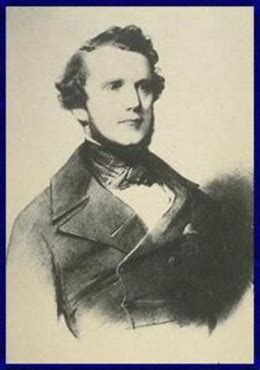
\includegraphics[scale=0.21]{bravais}
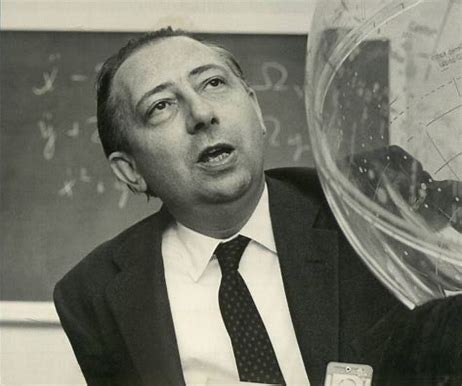
\includegraphics[scale=0.2]{wigner}
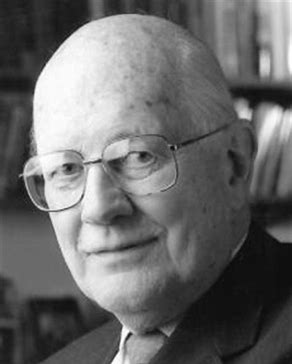
\includegraphics[scale=0.21]{seitz}
\end{figure}


\ech
\end{frame}

\begin{frame}
\frametitle{\bch 倒格 \ech}
\bch
给定由$\vec{a}_i$为基的布拉伐格$\Lambda$,找到另一组$\vec{b}_i$使得
$$
\vec{a}_i \cdot \vec{b}_j = 2\pi \delta_{ij}
$$
格点的集合
$$
\Lambda^{*}=\left\{\mathbf{k}=\sum n_{i} \mathbf{b}_{i}, n_{i} \in \mathbf{Z}\right\}
$$称为倒格。
\par

\ech
\end{frame}

\begin{frame}
\frametitle{\bch 倒矢 \ech}
\bch
试证明:
\begin{itemize}
\item 三维空间中的倒格的基底可以取成$\vec{b}_i = \frac{2\pi}{V} \frac{1}{2} \epsilon_{ijk} \vec{a}_j \times \vec{a}_k$;
\item 三个倒矢$\vec{b}_i$张成的体积为$\frac{(2\pi)^3}{V}$,其中$V$为元胞的体积;
\item 对任意布拉伐矢$\vec r$和倒矢$\vec q$,有$e^{i\vec q \cdot \vec r } =1$。
\end{itemize}
\ech
\end{frame}

\begin{frame}
\frametitle{\bch 三维布里渊区 \ech}
\bch
倒格的WS元胞称为布里渊区。
\cpic{0.4}{brillouin}
\ech
\end{frame}

\begin{frame}
\frametitle{\bch 课堂小练习 \ech}
\bch
画出下面的格矢构成的格点,画出它们的WS元胞;求它们的倒矢,画出前两个布里渊区。
\begin{itemize}
\item $\vec{a}_1$,$\vec{a}_2$长度均为$a$,夹角为$60^\circ$;
\item $\vec{a}_1$,$\vec{a}_2$长度均为$a$,夹角为$45^\circ$;
\item $\vec{a}_1$,$\vec{a}_2$长度分别为$a$,$3a$,夹角为$60^\circ$。
\end{itemize}
\ech
\end{frame}




\begin{frame}
\frametitle{\bch 三维格点上的离散傅立叶变换 \ech}
\bch
设函数$f(\vec x)$仅生活在布拉伐格$\vec{x} = n_1 \vec{a}_1 + n_2 \vec{a}_2 + n_3 \vec{a}_3$上,$f(n_1,n_2,n_3)$的傅立叶分解为
$$f(n_1,n_2,n_3) = \sum_{\vec k} f_{\vec k} e^{i\vec k \cdot \vec x}$$
PBC要求$f(\vec x) = f(\vec x + N_1 \vec{a}_1) = f(\vec x + N_2 \vec{a}_2) = f(\vec x + N_3 \vec{a}_3)$,其中$N_1,\ N_2,\ N_3$分别是沿三个布拉伐矢方向上的所有晶格数。
\par
证明,PBC要求
$$
\vec k = \frac{\ell_1}{N_1} \vec{b}_1 + \frac{\ell_2}{N_2} \vec{b}_2 + \frac{\ell_3}{N_3} \vec{b}_3
$$
其中$\vec{b}_i$是三个倒矢,$\ell_i= -\frac{N_i}{2},\cdots,\frac{N_i}{2} - 1$为整数。

\ech
\end{frame}

\begin{frame}
\frametitle{\bch 三维格点上的离散傅立叶变换 \ech}
\bch
证明:
\begin{itemize}
\item 基底$e^{i\vec k \cdot \vec x}$按
$$
\sum_{\vec{k}} (e^{i\vec k \cdot \vec x})^* e^{i\vec k \cdot \vec y} ={N_1 N_2 N_3}  \delta_{\vec x \vec y},\ \sum_{\vec x \in \Lambda} (e^{i\vec{k}'\cdot \vec x})^* e^{i \vec k \cdot \vec x} = {N_1 N_2 N_3} \delta_{\vec k \vec{k}'}
$$
正交归一化;
\item 若$f(\vec x)$的离散傅立叶变换为$f_{\vec k}$,则$f(\vec x + \vec d)$的离散傅立叶变换为$e^{i\vec k \cdot \vec d} f_{\vec k}$。 
\end{itemize}
\ech
\end{frame}

\begin{frame}
\frametitle{\bch 格点周期函数 \ech}
\bch
称函数$f(\vec x)$具有格点周期性,若对所有布拉伐矢$\vec r \in \Lambda$,都有
$$
f(\vec x + \vec r) = f(\vec x)
$$
现在$f$不仅仅生活在格点上。

\ech
\end{frame}


\begin{frame}
\frametitle{\bch 格点周期函数的傅立叶变换 \ech}
\bch
将空间按元胞划分,格点周期函数$f(\vec x)$的傅立叶变换
$$
\begin{aligned}
f(\vec k) &= \int d^3 \vec x f(\vec x) e^{-i\vec k \cdot \vec x} \\
&= \sum_{\vec r \in \Lambda} \int_{PC} d^3 \vec x e^{-i\vec k \cdot (\vec x + \vec r)} f(\vec x + \vec r) \\
&= \sum_{\vec r \in \Lambda} e^{-i\vec k \cdot \vec r} \int_{PC} d^3 \vec x e^{-i\vec k \cdot \vec x} f(\vec x)
\end{aligned}
$$
其中$PC$代表对单个元胞。可以看到,周期函数整体的傅立叶变换相当于对单个元胞作局部傅立叶变换再乘上因子$\varDelta (\vec k) = \sum_{\vec r \in \Lambda} e^{-i\vec k \cdot \vec r}
$。
求证:$$\varDelta(\vec k) = V^* \sum_{\vec q \in \Lambda^*} \delta(\vec k - \vec q)$$
\ech
\end{frame}

\begin{frame}
\frametitle{\bch 格点周期函数的傅立叶逆变换 \ech}
\bch
记在单个元胞内的傅立叶积分
$$
S(\vec k ) = \int_{PC} d^3 \vec x f(\vec x) e^{-i \vec k \cdot \vec x}
$$
求证,$f(\vec k)$的傅立叶逆变换为
$$
f(\vec x) \equiv \int \frac{d^3 k}{(2\pi)^3} f(\vec k) e^{i\vec k \cdot \vec x} = \frac{V^*}{(2\pi)^3} \sum_{\vec q \in \Lambda^*} S(\vec q)e^{i\vec q \cdot \vec x}
$$
\ech
\end{frame}

\section{3D Band Structure}
\secpage{晶体能带结构}{周期势作为微扰}


\begin{frame}
\frametitle{\bch 三维Bloch定理 \ech}
\bch
若势函数$V(\vec x)$为格点周期函数,$\psi(\vec x)$是对应薛定谔方程的解,则一定有
$$
\psi(\vec x) = e^{i\vec k \cdot \vec r} u_{\vec k} (\vec x)
$$
其中$u_{\vec k} (\vec x)$是一个格点周期函数。$\vec k$称作晶体动量,决定电子能量;可以根据需要将晶体动量限制在第一布里渊区,并将高动量模式的电子映回第一布里渊区。
\ech
\end{frame}

\begin{frame}
\frametitle{\bch 证明 \ech}
\bch
和一维的一样,不讲了。
\cpic{0.6}{self}
\ech
\end{frame}

\begin{frame}
\frametitle{\bch 准自由电子模型 \ech}
\bch
哈密顿量$H = \frac{\vec p^2}{2m} + V(\vec x)$,将周期势$V(\vec x)$作为微扰,按平面波解$| \vec k \rangle \sim e^{i \vec k \cdot \vec x}$展开,微扰矩阵元为$\langle \vec{k}' | V | \vec{k} \rangle$。根据三维格点傅立叶变换,求证:
\par
$\langle \vec{k}' | V | \vec{k} \rangle$非零当且仅当$\vec k - \vec{k}' = \vec q \in V^*$,其中$V^*$为倒格。
\par
解释:以动量$\vec k$运动的电子可以且只可以被晶格散射到相差一个倒矢$\vec q$的动量$\vec k + \vec q$。
\ech
\end{frame}

\begin{frame}
\frametitle{\bch 能带结构 \ech}
\bch
于是如1维情况一样:
\begin{itemize}
\item 低动量模式:不用作简并微扰,$E(\vec k) \sim \vec{k}^2$。
\item 布里渊区边界:当无微扰的能谱$E(\vec k + \vec q) = E(\vec k)$时微扰矩阵元出现,需要作简并微扰,此时$\vec{q}^2 + 2\vec k \cdot \vec q = 0$,$\vec k = - \frac{1}{2} \vec q + \vec{k}_\perp$,正好对应某个布里渊区的边界。能隙$2|V_{\vec q} |$出现。
\end{itemize}
\ech
\end{frame}

\begin{frame}
\frametitle{\bch 三维束缚模型 \ech}
\bch
跟一维一样的,懒得讲了。
\cpic{0.6}{self}
\ech
\end{frame}

\section{Summary}
\begin{frame}
\frametitle{\bch 总结 \ech}
\bch
\begin{itemize}
\item 晶体的能带结构是离散平移不变性的直接结果;
\item 在布里渊区的边缘,色散曲线出现间隙,导致导带和禁带的分离,能隙可以用简并微扰计算;
\item 远离布里渊区边界的低动量模式电子几乎不会感受到周期势的作用。
\end{itemize}
\ech
\end{frame}

\begin{frame}
\frametitle{\bch 没学懂 \ech}
\bch
\cpic{0.3}{not_understand}
凝聚态物理学太难了。
\ech
\end{frame}



\end{document}